\documentclass[10pt, a4paper, twocolumn]{article}

%%%%%%%%%%%%%%%%%%%%%%%%%%%%%%%%%%%%%%%%%
% Wenneker Article
% Structure Specification File
% Version 1.0 (28/2/17)
%
% This file originates from:
% http://www.LaTeXTemplates.com
%
% Authors:
% Frits Wenneker
% Vel (vel@LaTeXTemplates.com)
%
% License:
% CC BY-NC-SA 3.0 (http://creativecommons.org/licenses/by-nc-sa/3.0/)
%
%%%%%%%%%%%%%%%%%%%%%%%%%%%%%%%%%%%%%%%%%

%----------------------------------------------------------------------------------------
%	PACKAGES AND OTHER DOCUMENT CONFIGURATIONS
%----------------------------------------------------------------------------------------

\usepackage[english]{babel} % English language hyphenation

\usepackage{microtype} % Better typography

\usepackage{amsmath,amsfonts,amsthm} % Math packages for equations

\usepackage[svgnames]{xcolor} % Enabling colors by their 'svgnames'

\usepackage[hang, small, labelfont=bf, up, textfont=it]{caption} % Custom captions under/above tables and figures

\usepackage{booktabs} % Horizontal rules in tables

\usepackage{lastpage} % Used to determine the number of pages in the document (for "Page X of Total")

\usepackage{graphicx} % Required for adding images

\usepackage{enumitem} % Required for customising lists
\setlist{noitemsep} % Remove spacing between bullet/numbered list elements

\usepackage{sectsty} % Enables custom section titles
\allsectionsfont{\usefont{OT1}{phv}{b}{n}} % Change the font of all section commands (Helvetica)

%----------------------------------------------------------------------------------------
%	MARGINS AND SPACING
%----------------------------------------------------------------------------------------

\usepackage{geometry} % Required for adjusting page dimensions

\geometry{
	top=1cm, % Top margin
	bottom=1.5cm, % Bottom margin
	left=2cm, % Left margin
	right=2cm, % Right margin
	includehead, % Include space for a header
	includefoot, % Include space for a footer
	%showframe, % Uncomment to show how the type block is set on the page
}

\setlength{\columnsep}{7mm} % Column separation width

%----------------------------------------------------------------------------------------
%	FONTS
%----------------------------------------------------------------------------------------

\usepackage[T1]{fontenc} % Output font encoding for international characters
\usepackage[utf8]{inputenc} % Required for inputting international characters

\usepackage{XCharter} % Use the XCharter font

%----------------------------------------------------------------------------------------
%	HEADERS AND FOOTERS
%----------------------------------------------------------------------------------------

\usepackage{fancyhdr} % Needed to define custom headers/footers
\pagestyle{fancy} % Enables the custom headers/footers

\renewcommand{\headrulewidth}{0.0pt} % No header rule
\renewcommand{\footrulewidth}{0.4pt} % Thin footer rule

\renewcommand{\sectionmark}[1]{\markboth{#1}{}} % Removes the section number from the header when \leftmark is used

%\nouppercase\leftmark % Add this to one of the lines below if you want a section title in the header/footer

% Headers
\lhead{} % Left header
\chead{\textit{\thetitle}} % Center header - currently printing the article title
\rhead{} % Right header

% Footers
\lfoot{} % Left footer
\cfoot{} % Center footer
\rfoot{\footnotesize Page \thepage\ of \pageref{LastPage}} % Right footer, "Page 1 of 2"

\fancypagestyle{firstpage}{ % Page style for the first page with the title
	\fancyhf{}
	\renewcommand{\footrulewidth}{0pt} % Suppress footer rule
}

%----------------------------------------------------------------------------------------
%	TITLE SECTION
%----------------------------------------------------------------------------------------

\newcommand{\authorstyle}[1]{{\large\usefont{OT1}{phv}{b}{n}\color{DarkRed}#1}} % Authors style (Helvetica)

\newcommand{\institution}[1]{{\footnotesize\usefont{OT1}{phv}{m}{sl}\color{Black}#1}} % Institutions style (Helvetica)

\usepackage{titling} % Allows custom title configuration

\newcommand{\HorRule}{\color{DarkGoldenrod}\rule{\linewidth}{1pt}} % Defines the gold horizontal rule around the title

\pretitle{
	\vspace{-30pt} % Move the entire title section up
	\HorRule\vspace{10pt} % Horizontal rule before the title
	\fontsize{32}{36}\usefont{OT1}{phv}{b}{n}\selectfont % Helvetica
	\color{DarkRed} % Text colour for the title and author(s)
}

\posttitle{\par\vskip 15pt} % Whitespace under the title

\preauthor{} % Anything that will appear before \author is printed

\postauthor{ % Anything that will appear after \author is printed
	\vspace{10pt} % Space before the rule
	\par\HorRule % Horizontal rule after the title
	\vspace{20pt} % Space after the title section
}

%----------------------------------------------------------------------------------------
%	ABSTRACT
%----------------------------------------------------------------------------------------

\usepackage{lettrine} % Package to accentuate the first letter of the text (lettrine)
\usepackage{fix-cm}	% Fixes the height of the lettrine

\newcommand{\initial}[1]{ % Defines the command and style for the lettrine
	\lettrine[lines=3,findent=4pt,nindent=0pt]{% Lettrine takes up 3 lines, the text to the right of it is indented 4pt and further indenting of lines 2+ is stopped
		\color{DarkGoldenrod}% Lettrine colour
		{#1}% The letter
	}{}%
}

\usepackage{xstring} % Required for string manipulation

\newcommand{\lettrineabstract}[1]{
	\StrLeft{#1}{1}[\firstletter] % Capture the first letter of the abstract for the lettrine
	\initial{\firstletter}\textbf{\StrGobbleLeft{#1}{1}} % Print the abstract with the first letter as a lettrine and the rest in bold
}

%----------------------------------------------------------------------------------------
%	BIBLIOGRAPHY
%----------------------------------------------------------------------------------------

\usepackage[backend=bibtex,style=authoryear,natbib=true]{biblatex} % Use the bibtex backend with the authoryear citation style (which resembles APA)

\addbibresource{example.bib} % The filename of the bibliography

\usepackage[autostyle=true]{csquotes} % Required to generate language-dependent quotes in the bibliography

\title{JavaScript}

\author{
	\authorstyle{Boitumelo Phetla\textsuperscript{1}} % Authors
	\newline\newline % Space before institutions
	\textsuperscript{1}\institution{PluralSight Google ScholarShip}
}


\date{\today} % Add a date here if you would like one to appear underneath the title block, use \today for the current date, leave empty for no date


\begin{document}
\maketitle % Print the title
\thispagestyle{firstpage} % Apply the page style for the first page (no headers and footers)

%----------------------------------------------------------------------------------------
%	ABSTRACT
%----------------------------------------------------------------------------------------

\lettrineabstract{JavaScript,  is a lightweight interpreted or just-in-time compiled programming language with first-class functions. While it is most well-known as the scripting language for Web pages, many non-browser environments also use it, such as Node.js, Apache CouchDB and Adobe Acrobat.}

%----------------------------------------------------------------------------------------
%	ARTICLE CONTENTS
%----------------------------------------------------------------------------------------

\section{Simplistic JavaScript 1}

\subsection{Command-line based programming}

A simple project:

\begin{lstlisting}

$bash: touch {index.html,script.js,style.css}
$bash: tree
	__________	index.html
	__________	script.js
	__________	style.css


\end{lstlisting}

Include the script (\textbf{javascript}) and the page styling script (\textbf{cascading stylesheet}) files into the \textit{index.html}.

\begin{lstlisting}
<!DOCTYPE>
	<html>
		<head>
				<script src="path/*.js"></script>
				<link rel="stylesheet" href="path/*.css">
		</head>
				<body>
						<div>
								<header></header>
						</div>
							<div><!-- body --></div>
						<div>
							<footer></footer>
						</div>
				</body>
	</html>

\end{lstlisting}

Add some simple HTML markup code and launch a live-server of the code.

\begin{lstlisting}
	<!DOCTYPE>
	<html>
			<head>
					<script src="script.js"></script>
					<link rel="stylesheet" href="style.css">
			</head>
					<body>
							<div id="header">
									<h1>Welcome to JavaScript</h1>
							</div>
					</body>
	</html>
\end{lstlisting}

Launch the command-line (Terminal)

\begin{lstlisting}
$bash: live-server
\end{lstlisting}

\begin{figure}[h!]
	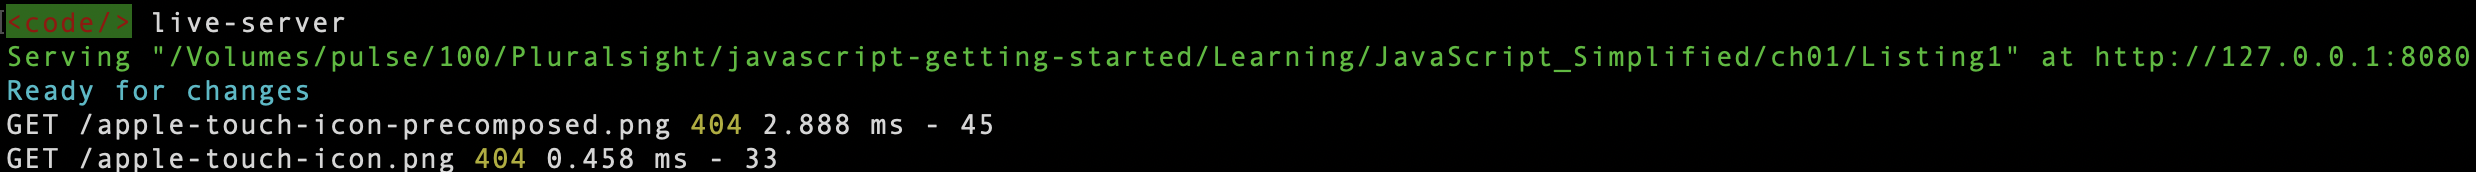
\includegraphics[width=\linewidth]{liveserver.png} % Figure image
	\caption{Live-server} % Figure caption
	\label{ls} % Label for referencing with \ref{bear}
\end{figure}

\newpage
\subsection{\href{http://plnkr.co}{Plunker}}

Or create an account on  \href{http://plnkr.co/edit/?p=catalogue}{Plunker}.  Plunker sets up your working environment for you.

\begin{figure}[h!]
	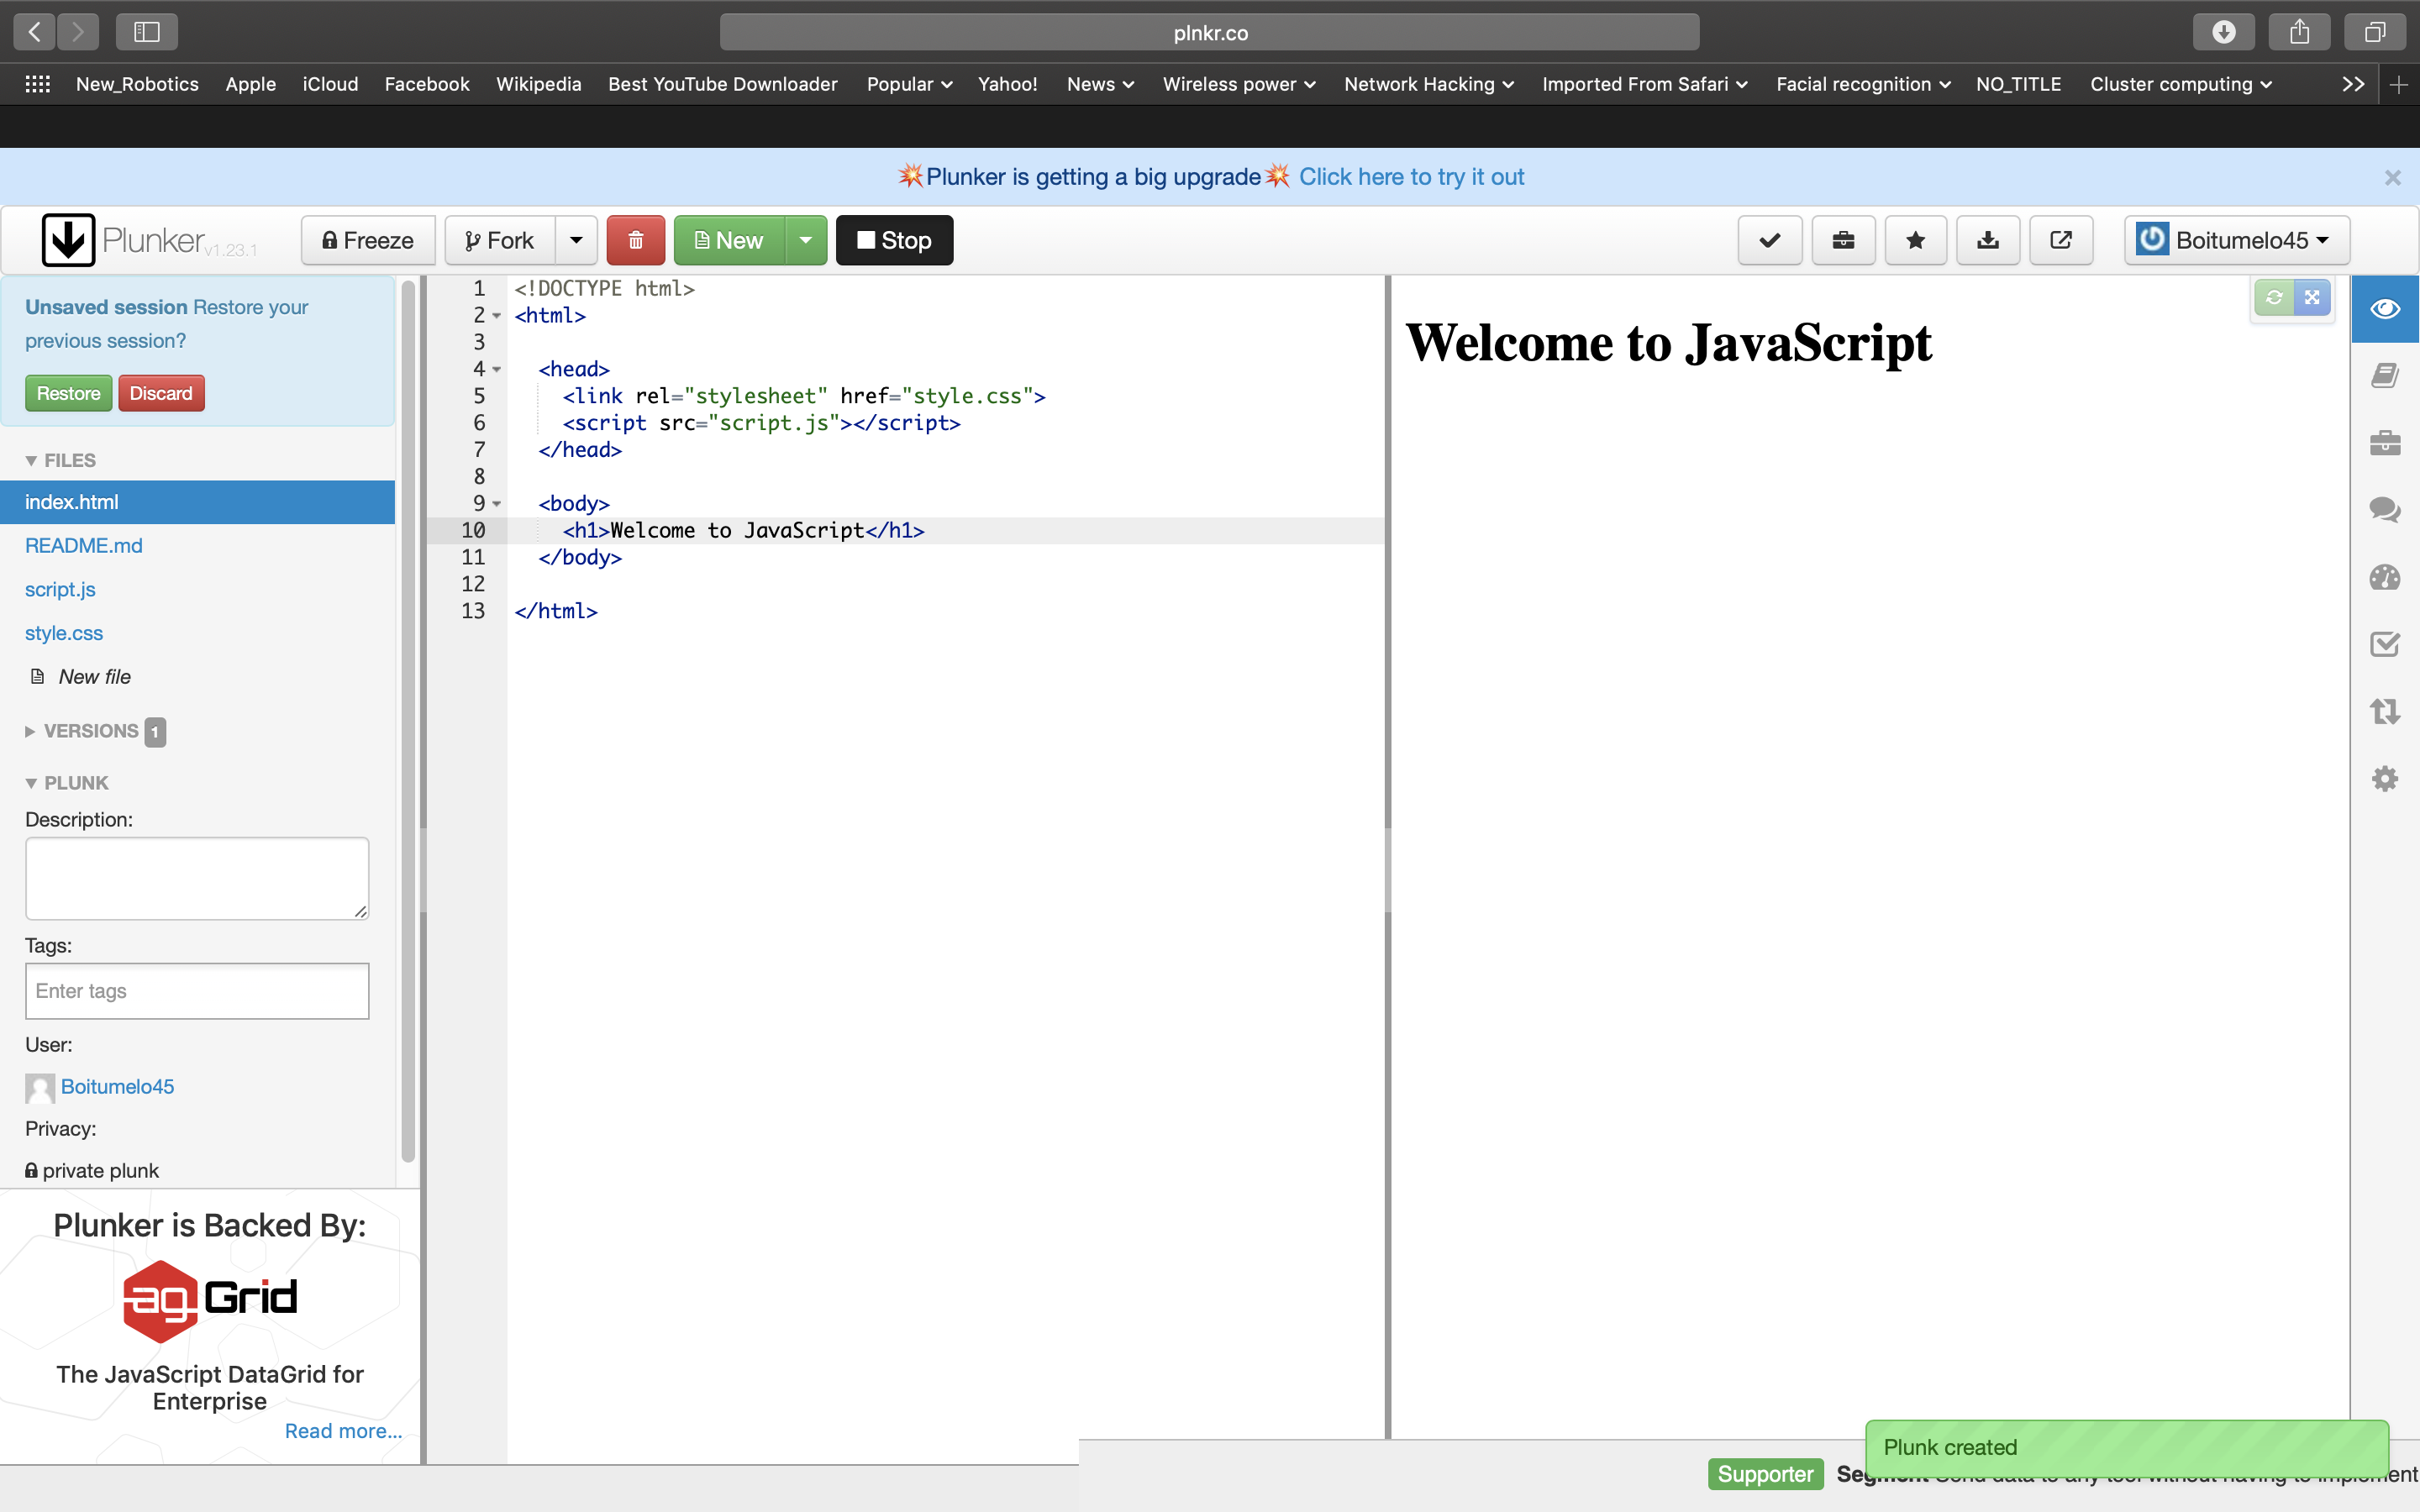
\includegraphics[width=\linewidth]{plunker.png} % Figure image
	\caption{Plunker} % Figure caption
	\label{plnkr} % Label for referencing with \ref{bear}
\end{figure}

\subsection{\href{https://electronjs.org}{Electron}}

Watch this video \href{https://www.youtube.com/watch?v=8YP_nOCO-4Q&feature=youtu.be}{Electron}.

\begin{lstlisting}
# Clone the Quick Start repository
$ git clone https://github.com/electron/electron-quick-start

# Go into the repository
$ cd electron-quick-start

# Install the dependencies and run
$ npm install && npm start
\end{lstlisting}

\begin{figure}[h!]
	
\includegraphics[width=\linewidth]{electron.png} % Figure image
	\caption{Electron} % Figure caption
	\label{elec} % Label for referencing with \ref{bear}
\end{figure}

\begin{lstlisting}
$bash: mkdir Electron1; cd Electron1; npm init
  1 {
  2   "name": "electron1",
  3   "version": "1.0.0",
  4   "description": "First App",
  5   "main": "index.js",
  6   "scripts": {
  7     "test": "echo \"Error: no test specified\" && exit 1"
  8   },
  9   "keywords": [
 10     "Electron"
 11   ],
 12   "author": "Boitumelo Phetla",
 13   "license": "ISC"
 14 }
\end{lstlisting}

At this point, you'll need to install electron itself. The recommended way of doing so is to install it as a development dependency in your app, which allows you to work on multiple apps with different Electron versions. To do so, run the following command from your app's directory:

\begin{lstlisting}
$bash: npm install --save-dev electron
$bash: tree -L 1
			.
			|____________node_modules
			|____________package-lock.json
			|____________package.json

1 directory, 2 files
\end{lstlisting}

All APIs and features found in Electron are accessible through the electron module, which can be required like any other Node.js module:

\begin{lstlisting}
const electron = require('electron')
\end{lstlisting}

To avoid any huddles, try this simple example.

\begin{lstlisting}
# Clone the repository
$ git clone https://github.com/electron/electron-quick-start
# Go into the repository
$ cd electron-quick-start
# Install dependencies
$ npm install
# Run the app
$ npm start
\end{lstlisting}

\subsection{\href{https://www.meteor.com/install}{Meteor}}


\begin{figure}[h!]
	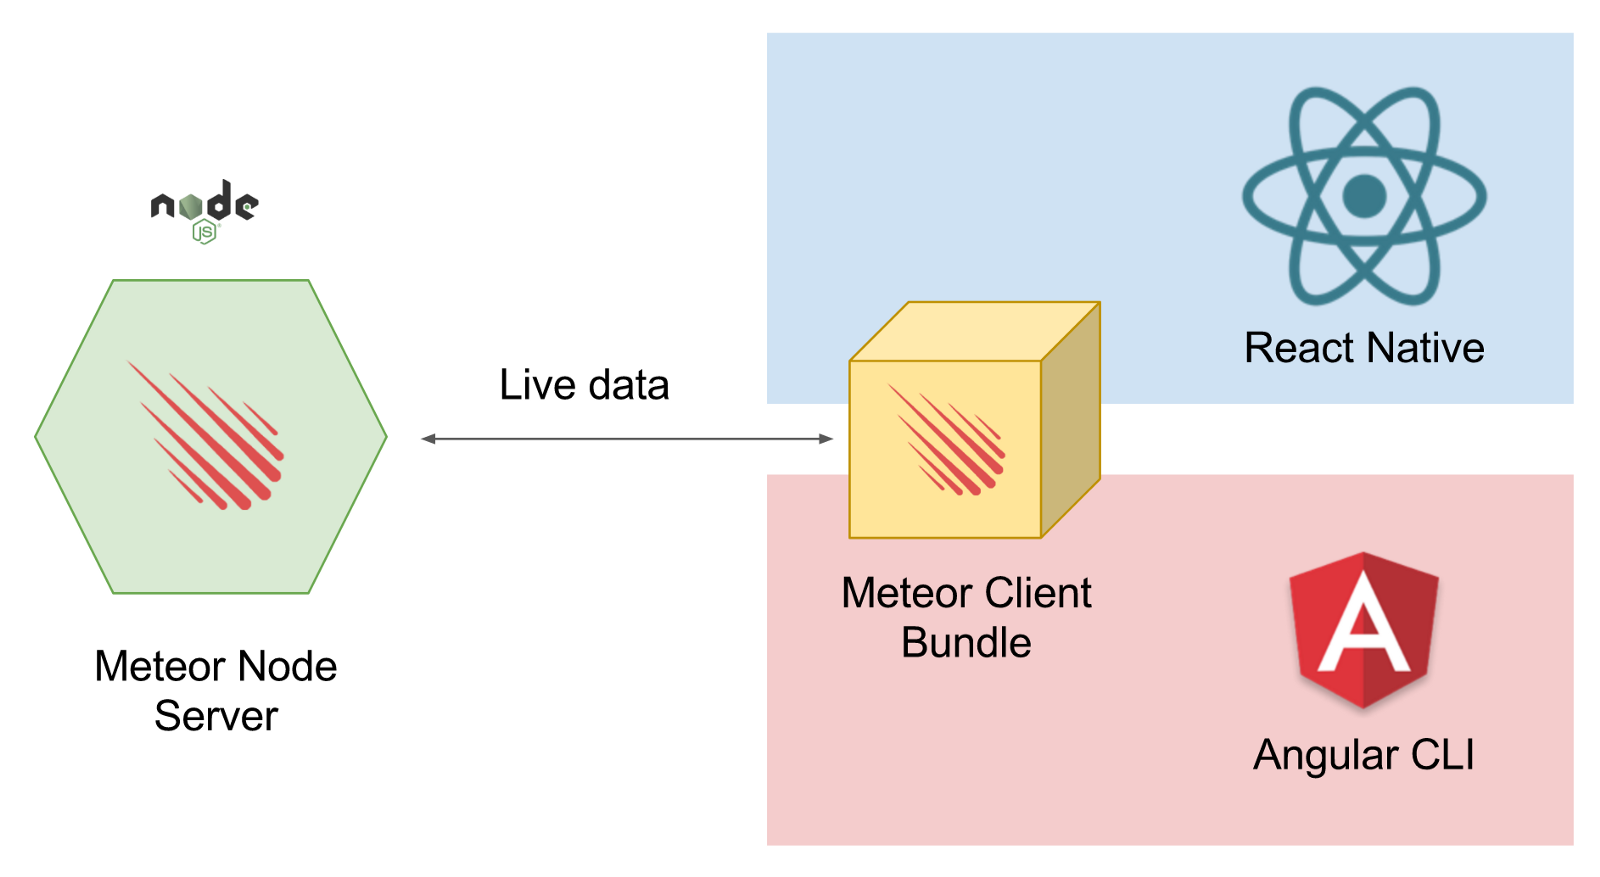
\includegraphics[width=\linewidth]{meteor.png} % Figure image
	\caption{Meteor} % Figure caption
	\label{mtr} % Label for referencing with \ref{bear}
\end{figure}

To create the app, open your terminal and type:

\begin{lstlisting}
$bash: meteor create simple-todos

output:

Created a new Meteor app in 'simple-todos'.

To run your new app:
  cd simple-todos
  meteor

If you are new to Meteor, try some of the learning resources here:
  https://www.meteor.com/tutorials

To start with a different app template, try one of the following:

  meteor create --bare    # to create an empty app
  meteor create --minimal # to create an app with as few Meteor packages as possible
  meteor create --full    # to create a more complete scaffolded app

\end{lstlisting}


%------------------------------------------------

\subsection{Coding in JavaScript}

\subsubsection{Variables}

\begin{lstlisting}
"use strict";
//let is accessible in the code block where it is used
let firstName = "John Doe"; //camelCasing
console.log(firstName);

/*Output*/
$bash: node let.js
John Doe
\end{lstlisting}

\subsubsection{Global variable, function, Operators}
\begin{lstlisting}
"use strict";

//A = P(1 + rt)
let r = 10.5, t = 5, p = 200;

var A = (r,t,p) => {
  return p*(1 + (r/100)*t);
}

let interest = A(r,t,p);
console.log("R200 (interest in 5 years at at interest rate of 10.5% = R" + interest + "-00)");

\end{lstlisting}

\subsubsection{Simple function}

\begin{lstlisting}
"use strict";

//A = P(1 + rt)
let r = 10.5, t = 5, p = 200;

//function definition (without using arrow function)
var A = function(r,t,p){
    return p*(1 + (r/100)*t);
}

console.log(A(r,t,p));

\end{lstlisting}

\subsubsection{Variables and block code}

\begin{lstlisting}
"use strict";

array = [1,2,3,4,5];
var count = 0;
let counter = 0;

for(let i = 0; i < array.length; i++){
    count += array[i];
    counter += i;
    if(count > 5){
        var num1 = count*5;     //accessible outside this code block
        let num2 = num1*5;      //only accessible within this code block
        console.log("num1: ", num1, ',', 'num2: ', num2);
    }
    //console.log("xnum1: ", num1, ',', 'xnum2: ', num2);
    try{
        console.log("xnum1: ", num1, ',', 'xnum2: ', num2);
    }catch{
        console.log('xnum1: ', num1);   //<-- accessing num1
        console.log('xnum2: ', 'This will not print because it is not accessible'); //<-- can't access num2
    }

}
console.log('count: ', count, ',' , 'counter: ',counter); //<-- both count and counter are accessible because they are in the same code block

/*Output*/
xnum1:  undefined
xnum2:  This will not print because it is not accessible
xnum1:  undefined
xnum2:  This will not print because it is not accessible
num1:  30 , num2:  150
xnum1:  30
xnum2:  This will not print because it is not accessible
num1:  50 , num2:  250
xnum1:  50
xnum2:  This will not print because it is not accessible
num1:  75 , num2:  375
xnum1:  75
xnum2:  This will not print because it is not accessible
count:  15 , counter:  10
\end{lstlisting}

\subsubsection{Type of primitive data}

\begin{lstlisting}
"use strict";

let b  = false;
let array = [1,2,3,'hello', 3.02,  b];

var typeOfData = (array) =>{
  array.forEach((element) =>{
    console.log(element, 'is a ', typeof(element));
  })
}

typeOfData(array);

/*Output*/

1 'is a ' 'number'
2 'is a ' 'number'
3 'is a ' 'number'
hello is a  string
3.02 'is a ' 'number'
false 'is a ' 'boolean'

\end{lstlisting}

\subsubsection{Undefined and Null}

\begin{lstlisting}
"use strict";

let anUndefinedVariable;  //not initialized
let empty = null; //is empty (nothing)

console.log(anUndefinedVariable, empty);
console.log(typeof(anUndefinedVariable), typeof(empty));

/*Output*/

undefined null
undefined object

\end{lstlisting}

\subsubsection{Data containers}


\textbf{Array}

\begin{lstlisting}
"use strict";

/*
  We use arrays to contain multiple variables values instead of declaring a thousand of them.
*/

let array = ["John", "Doe", 34, "X", "USA", "Nevada", "Porsche 911", ["soccer", "volleyball", "chess"], ["python", "nim", "c", "java", "julia", "objective C", "SQL", "GraphQL", "JavaScript", "HTML5", "CSS3", "jQuery", "Machine Learning", "Bash"],"MIT", "In a relationship", ["Bali", "Singapore", "Hong Kong", "Thailand", "Mozambique", "Swaziland", "South Africa", "Lombark"], ["Electrical", "Computer"]];

array.forEach((element)=>{console.log(element)});

/*Output*/

John
Doe
34
X
USA
Nevada
Porsche 911
[ 'soccer', 'volleyball', 'chess' ]
[ 'python',
  'nim',
  'c',
  'java',
  'julia',
  'objective C',
  'SQL',
  'GraphQL',
  'JavaScript',
  'HTML5',
  'CSS3',
  'jQuery',
  'Machine Learning',
  'Bash' ]
MIT
In a relationship
[ 'Bali',
  'Singapore',
  'Hong Kong',
  'Thailand',
  'Mozambique',
  'Swaziland',
  'South Africa',
  'Lombark' ]
[ 'Electrical', 'Computer' ]

\end{lstlisting}

Add values into an empty array

\begin{lstlisting}
"use strict";

/*
  We use arrays to contain multiple variables values instead of declaring a thousand of them.
*/

let array = ["John", "Doe", 34, "X", "USA", "Nevada", "Porsche 911"];
let results = [] //empty array

/*
  add elements into array
  array.push(value)
*/

for(let i = 0; i < array.length; i++){
    results.push(array[i]);
}

console.log("Length of results[]: ", results.length);
console.log(results);

/*Output*/
Length of results[]:  7
[ 'John', 'Doe', 34, 'X', 'USA', 'Nevada', 'Porsche 911' ]

\end{lstlisting}


Removing elements from an array

\begin{lstlisting}
"use strict";

let array = ["John", "Doe", 34, "X", "USA", "Nevada", "Porsche 911"];
/*
 remove elements from an array
 array.pop(); //removes last value
*/
while(array.length > 0){
        array.pop();
}

console.log("Length of array: ", array.length);
console.log(array);

/*Output*/
Length of array:  0
[]

\end{lstlisting}

Removing the first elements by shifting the array.

\begin{lstlisting}

"use strict";

let array = ["John", "Doe", 34, "X", "USA", "Nevada", "Porsche 911"];
array.shift(); //shifts the array

console.log(array);

/*Output*/

[ 'Doe', 34, 'X', 'USA', 'Nevada', 'Porsche 911' ]

\end{lstlisting}

Deleting elements from an array.

\begin{lstlisting}
"use strict";

let array = ["cobol", "c#", ".NET", "Python"];

/*
  delete the first three elements of the array
*/

let languages_depricated = array.splice(0,3);
console.log(array, languages_depricated);

/*Output*/
[ 'Python' ] [ 'cobol', 'c#', '.NET' ]
\end{lstlisting}

Deleting elements from an array and mutating it.

\begin{lstlisting}
"use strict";

let array = ["cobol", "c#", ".NET", "Python"];

/*
  delete the first three elements of the array and mutating the array
  using splice()

	splice(0,3) - means:
	delete element from index 0 and delete 3 items
	if array = [1,2,3,4]
	splice(0,3)
			performs:
							[2,3,4]  - 1 : delete[1]
							[3,4] - 2 : delete[2]
							[4] - 3 : delete[3]
							all at index 0
			returns new array = [4]
*/

let deleted = array.splice(0,3, "Java", "C", "Nim", "Objective C", "Swing");
console.log(array, deleted);

/*Output*/
[ 'Java', 'C', 'Nim', 'Objective C', 'Swing', 'Python' ] [ 'cobol', 'c#', '.NET' ]
\end{lstlisting}

Some of Array methods you can use.

\begin{description}[align=left]
\item [forEach()] This method can help you to loop over array's items.
\begin{lstlisting}
const arr = [1, 2, 3, 4, 5, 6];

  arr.forEach(item => {
    console.log(item); // output: 1 2 3 4 5 6
  });
\end{lstlisting}
\item [includes()] This method check if array includes the item passed in the method.
\begin{lstlisting}
const arr = [1, 2, 3, 4, 5, 6];

 arr.includes(2); // output: true
 arr.includes(7); // output: false
\end{lstlisting}
\item [filter()] This method create new array with only elements passed condition inside the provided function.
\begin{lstlisting}
const arr = [1, 2, 3, 4, 5, 6];

  // item(s) greater than 3
  const filtered = arr.filter(num => num > 3);
  console.log(filtered); // output: [4, 5, 6]

  console.log(arr); // output: [1, 2, 3, 4, 5, 6]
\end{lstlisting}
\item [map()] This method create new array by calling the provided function in every element.The reduce() method applies a function against an accumulator and each element in the array (from left to right) to reduce it to a single value - MDN
\begin{lstlisting}
const arr = [1, 2, 3, 4, 5, 6];

 // add one to every element
 const oneAdded = arr.map(num => num + 1);
 console.log(oneAdded); // output [2, 3, 4, 5, 6, 7]

 console.log(arr); // output: [1, 2, 3, 4, 5, 6]
\end{lstlisting}
\item [reduce()] This method check if at least one of array's item passed the condition. If passed, it return 'true' otherwise 'false'.
\begin{lstlisting}
const arr = [1, 2, 3, 4, 5, 6];

 const sum = arr.reduce((total, value) => total + value, 0);
 console.log(sum); // 21
\end{lstlisting}
\item [some()] This method check if at least one of array's item passed the condition. If passed, it return 'true' otherwise 'false'.
\begin{lstlisting}
const arr = [1, 2, 3, 4, 5, 6];

// at least one element is greater than 4?
const largeNum = arr.some(num => num > 4);
console.log(largeNum); // output: true

// at least one element is less than or equal to 0?
const smallNum = arr.some(num => num <= 0);
console.log(smallNum); // output: false
\end{lstlisting}
\item [every()] This method check if all array's item passed the condition. If passed, it return 'true' otherwise 'false'.
\begin{lstlisting}
const arr = [1, 2, 3, 4, 5, 6];

  // all elements are greater than 4
  const greaterFour = arr.every(num => num > 4);
  console.log(greaterFour); // output: false

  // all elements are less than 10
  const lessTen = arr.every(num => num < 10);
  console.log(lessTen); // output: true
\end{lstlisting}
\item [sort()] This method used to arrange/sort array's item either ascending or descending order.
\begin{lstlisting}
const arr = [1, 2, 3, 4, 5, 6];
const alpha = ['e', 'a', 'c', 'u', 'y'];

// sort in descending order
descOrder = arr.sort((a, b) => a > b ? -1 : 1);
console.log(descOrder); // output: [6, 5, 4, 3, 2, 1]

// sort in ascending order
ascOrder = alpha.sort((a, b) => a > b ? 1 : -1);
console.log(ascOrder); // output: ['a', 'c', 'e', 'u', 'y']
\end{lstlisting}
\item [Array.from()] This change all thing that are array-like or iterable into true array especially when working with DOM, so that you can use other array methods like reduce, map, filter and so on.
\newline\newline
code 1
\begin{lstlisting}
const name = 'frugence';
const nameArray = Array.from(name);

console.log(name); // output: frugence
console.log(nameArray); // output: ['f', 'r', 'u', 'g', 'e', 'n', 'c', 'e']
\end{lstlisting}
code 2
\begin{lstlisting}
// I assume that you have created unorder list of items in our html file.

const lis = document.querySelectorAll('li');
const lisArray = Array.from(document.querySelectorAll('li'));

// is true array?
console.log(Array.isArray(lis)); // output: false
console.log(Array.isArray(lisArray));  // output: true
\end{lstlisting}
\item [Array.of()] This create array from every arguments passed into it.
\begin{lstlisting}
const nums = Array.of(1, 2, 3, 4, 5, 6);
console.log(nums); // output: [1, 2, 3, 4, 5, 6]
\end{lstlisting}
\end{description}

\newpage
\textbf{Dictionary}

\begin{lstlisting}

"use strict";

let data  = {

    "first name": "John",
    "last name" : "Doe",
    "age"       : 34,
    "company"   : "X",
    "country"   : "USA",
    "State"     : "Nevada",
    "car"       : "Porsche 911",
    "hobby"     : ["soccer", "volleyball", "chess"],
    "polyglot"  : ["python", "nim", "c", "java", "julia", "objective C", "SQL", "GraphQL", "JavaScript", "HTML5", "CSS3", "jQuery", "Machine Learning", "Bash"],
    "university" : "MIT",
    "status"     : "in a relationship",
    "travels"    : ["Bali", "Singapore", "Hong Kong", "Thailand", "Mozambique", "Swaziland", "South Africa", "Lombark"],
    "Degrees"   : ["Electrical", "Computer"]


}

console.log(data);


/*Output*/

{ 'first name': 'John',
  'last name': 'Doe',
  age: 34,
  company: 'X',
  country: 'USA',
  State: 'Nevada',
  car: 'Porsche 911',
  hobby: [ 'soccer', 'volleyball', 'chess' ],
  polyglot:
   [ 'python',
     'nim',
     'c',
     'java',
     'julia',
     'objective C',
     'SQL',
     'GraphQL',
     'JavaScript',
     'HTML5',
     'CSS3',
     'jQuery',
     'Machine Learning',
     'Bash' ],
  university: 'MIT',
  status: 'in a relationship',
  travels:
   [ 'Bali',
     'Singapore',
     'Hong Kong',
     'Thailand',
     'Mozambique',
     'Swaziland',
     'South Africa',
     'Lombark' ],
  Degrees: [ 'Electrical', 'Computer' ] }

\end{lstlisting}


\subsubsection{Blackjack project (PluralSight)}

\begin{lstlisting}
/*
  Blackjack game of cards
*/

let card1 = "Ace of Spades", card2 = "Ten of hearts";
let cards = [card1, card2];

console.log("Welcome to Blackjack");
console.log("You are dealt: ");
cards.forEach((element) => {
    console.log("\t" + element);
})

/*Output*/
Welcome to Blackjack
You are dealt:
        Ace of Spades
        Ten of hearts
\end{lstlisting}

For loops, Arrays

\begin{lstlisting}
/*
  Blackjack game of cards
*/

let suits = ["Heart", "Clubs", "Diamonds", "Spades"];
let values = ["Ace", "King", "Queen", "Jack", "Ten", "Nine", "Eight", "Seven", "Six", "Five", "Four", "Three", "Two"];


let deck = []

for(let suitIdx = 0; suitIdx < suits.length; suitIdx++){
    for(let valueIdx = 0; valueIdx < values.length; valueIdx++){
        deck.push(values[valueIdx] + ' of ' + suits[suitIdx]);
    }
}

console.log(deck);

/*Output*/
....
 'Four of Spades',
 'Three of Spades',
 'Two of Spades' ]
\end{lstlisting}

Advancing the Blackjack code.

\begin{lstlisting}
/*
Blackjack game of cards
*/

let suits = ["Heart", "Clubs", "Diamonds", "Spades"];
let values = ["Ace", "King", "Queen", "Jack", "Ten", "Nine", "Eight", "Seven", "Six", "Five", "Four", "Three", "Two"];


function createDeck(){
	let deck = [] //crear deck
	for(let suitIdx = 0; suitIdx < suits.length; suitIdx++){
			for(let valueIdx = 0; valueIdx < values.length; valueIdx++){
					deck.push(values[valueIdx] + ' of ' + suits[suitIdx]);
			}
	}
			return deck
}

let deck = createDeck()
//console.log(deck);

function getNextCard(){
	return deck.shift()
}


let playerCards = []

for(let i = 0; i < 2; i++){
	playerCards.push(getNextCard())
}

console.log(playerCards);

\end{lstlisting}

Objects and functions in the code.

\begin{lstlisting}
/*
Blackjack game of cards
*/

let suits = ["Heart", "Clubs", "Diamonds", "Spades"];
let values = ["Ace", "King", "Queen", "Jack", "Ten", "Nine", "Eight", "Seven", "Six", "Five", "Four", "Three", "Two"];


function createDeck(){
	let deck = [] //crear deck
	for(let suitIdx = 0; suitIdx < suits.length; suitIdx++){
			for(let valueIdx = 0; valueIdx < values.length; valueIdx++){
					deck.push(values[valueIdx] + ' of ' + suits[suitIdx]);
			}
	}
			return deck
}

let deck = createDeck()
//console.log(deck);

function getNextCard(){
	return deck.shift()
}


let playerCards = []

for(let i = 0; i < 2; i++){
	playerCards.push(getNextCard())
}

console.log(playerCards);
\end{lstlisting}

Objects

\begin{lstlisting}
/*
Blackjack game of cards
*/

let suits = ["Heart", "Clubs", "Diamonds", "Spades"];
let values = ["Ace", "King", "Queen", "Jack", "Ten", "Nine", "Eight", "Seven", "Six", "Five", "Four", "Three", "Two"];


function createDeck(){
	/*
			Creates a deck of 52 cards
	*/
	let deck = [] //crear deck
	for(let suitIdx = 0; suitIdx < suits.length; suitIdx++){
			for(let valueIdx = 0; valueIdx < values.length; valueIdx++){
					let card = {
									suit : suits[suitIdx],
									value: values[valueIdx]
					}
					deck.push(card);
			}
	}
			return deck
}

let deck = createDeck()
//console.log(deck);

function getNextCard(){
	/*Moves to the next card from the card on top*/
	return deck.shift()
}

var getCardString = (card) =>{
	/*
			takes object { suit: "v1", valueL "v2"}
			returns: v2 of v1
	*/
	return card.value + ' of ' + card.suit
}

let playerCards = []

for(let i = 0; i < 2; i++){
	playerCards.push(getCardString(getNextCard()))
}

console.log("Welcome to BlackJack Game!");
console.log("You are dealt: ");
console.log(playerCards);
\end{lstlisting}

\subsection{Adding user interface to BlackJack Game}

\begin{description}
	\item[HTML file]: /interface/listing1/listing1.html
\end{description}

\begin{lstlisting}
<!DOCTYPE html>
<!DOCTYPE html>
<html>
	<head>
		<meta charset="utf-8">
		<title>BlackJack!</title>
	</head>
	<body>
				<h1>BlackJack</h1>
				<h4>By Boitumelo Phetla</h4>
				<hr>
				<br>
				<p id="text-area">Welcome to BlackJack</p>
				<button type="button" name="button1" id="new-game-button">New Game!</button>
				<button type="button" name="button2" id="hit-button">Hit!</button>
				<button type="button" name="button3" id="stay-button">Stay</button>
				<script src="blackjackFn4.js"></script>
	</body>
</html>
\end{lstlisting}

\begin{description}
	\item[JS file]:  /interface/listing1/blackjackFn4.js
\end{description}

\begin{lstlisting}
/*
	Blackjack game of cards
*/

let suits = ["Heart", "Clubs", "Diamonds", "Spades"];
let values = ["Ace", "King", "Queen", "Jack", "Ten", "Nine", "Eight", "Seven", "Six", "Five", "Four", "Three", "Two"];

let textArea = document.getElementById('text-area')
let newGameButton = document.getElementById('new-game-button')
let hitButton = document.getElementById('hit-button')
let stayButton = document.getElementById('stay-button')

function hide(object){
		object.style.display = 'none' //remove element
}

function unhide(object){
		object.style.display = 'inline' //revert back
}

function newGame(textObject, newGameButtonObject, hitButtonObject, stayButtonObject){
		textObject.innerText = "Started..."
		//hide newGameButton
		hide(newGameButtonObject)
		//unhide stay and hit button
		unhide(hitButtonObject)
		unhide(stayButtonObject)
}
//start hide hit and stay button
hide(hitButton)
hide(stayButton)

newGameButton.addEventListener('click', function(){
		newGame(textArea, newGameButton, hitButton, stayButton)
})

function createDeck(){
		/*
				Creates a deck of 52 cards
		*/
		let deck = [] //crear deck
		for(let suitIdx = 0; suitIdx < suits.length; suitIdx++){
				for(let valueIdx = 0; valueIdx < values.length; valueIdx++){
						let card = {
										suit : suits[suitIdx],
										value: values[valueIdx]
						}
						deck.push(card);
				}
		}
				return deck
}

let deck = createDeck()
//console.log(deck);

function getNextCard(){
		/*Moves to the next card from the card on top*/
		return deck.shift()
}

var getCardString = (card) =>{
		/*
				takes object { suit: "v1", valueL "v2"}
				returns: v2 of v1
		*/
		return card.value + ' of ' + card.suit
}

let playerCards = []

for(let i = 0; i < 2; i++){
		playerCards.push(getCardString(getNextCard()))
}

console.log("Welcome to BlackJack Game!");
console.log("You are dealt: ");
console.log(playerCards);
\end{lstlisting}

\subsection{Adding game functionalities}

\begin{lstlisting}
/*
	Blackjack game of cards
*/

//Game variables
let gameStarted = false, gameOver = false, playerWon = false, dealerCards = [], playerCards = [], dealerScore = 0, playerScore = 0, deck = []

//card variables
let suits = ["Heart", "Clubs", "Diamonds", "Spades"];
let values = ["Ace", "King", "Queen", "Jack", "Ten", "Nine", "Eight", "Seven", "Six", "Five", "Four", "Three", "Two"];

//DOM variables
let textArea = document.getElementById('text-area')
let newGameButton = document.getElementById('new-game-button')
let hitButton = document.getElementById('hit-button')
let stayButton = document.getElementById('stay-button')

//create deck function
function createDeck(){
		/*
				Creates a deck of 52 cards
		*/
		let deck = [] //crear deck
		for(let suitIdx = 0; suitIdx < suits.length; suitIdx++){
				for(let valueIdx = 0; valueIdx < values.length; valueIdx++){
						let card = {
										suit : suits[suitIdx],
										value: values[valueIdx]
						}
						deck.push(card);
				}
		}
				return deck
}

function getNextCard(){
		/*Moves to the next card from the card on top*/
		return deck.shift()
}

var getCardString = (card) =>{
		/*
				takes object { suit: "v1", valueL "v2"}
				returns: v2 of v1
		*/
		return card.value + ' of ' + card.suit
}

function hide(object){
		object.style.display = 'none' //remove element
}

function unhide(object){
		object.style.display = 'inline' //revert back
}

function getCardNumericValue(card){
		switch(card.value){
				case 'Ace':
						return 1
				case 'Two':
						return 2
				case 'Three':
						return 3
				case 'Four':
						return 4
				case 'Five':
						return 5
				case 'Six':
						return 6
				case 'Seven':
						return 7
				case 'Eight':
						return 8
				case 'Nine':
						return 9
				default:
						return 10
		}
}

function updateScore(){
		dealerScore = getScore(dealerCards)
		playerScore = getScore(playerCards)
}

function getScore(cardArray){
		let score = 0
		let hasAce = false
		for (var i = 0; i < cardArray.length; i++) {
				let card = cardArray[i]
				console.log(card);
				score += getCardNumericValue(card)
				if(card.value === 'Ace'){
						hasAce = true
				}
		}
		if(hasAce && score + 10 <= 21){
				return score + 10
		}

		return score
}

function showStatus(){
		if(!gameStarted){
				textArea.innerText = "Welcome to BlackJack!"
				return;
		}

		console.log("Debugging")
		console.log(dealerCards, playerCards) //debugging

		let dealerCardString = ''
		console.log("Dealer cards:");
		for (let i = 0; i < dealerCards.length; i++) {
				dealerCardString += getCardString(dealerCards[i]) + '\n'
				console.log(dealerCards[i])
		}

		let playerCardString = ''
		console.log("Player cards:");
		for (let i = 0; i < playerCards.length; i++) {
				playerCardString += getCardString(playerCards[i]) + '\n'
				console.log(playerCards[i])
		}

		updateScore()

		textArea.innerText =
				'Dealer has:\n' +
				dealerCardString +
				'(score: ' + dealerScore + ')\n\n'+

				'Player has:\n' +
				playerCardString +
				'(score: ' + playerScore + ')\n\n'

		if(gameOver){
				if(playerWon){
						textArea.innerText = "You WIN!"
				}else{
						textArea.innerText = "DEALER WINS!"
				}

				unhide(newGameButton)
				hide(hitButton)
				hide(stayButton)
		}


}

//shuffle deck
function shuffleDeck(deckOfCards){
		for(let i = 0; i < deckOfCards.length; i++){
				let swapIdx = Math.trunc(Math.random()* deckOfCards.length)
				let tmp = deckOfCards[swapIdx];
				deckOfCards[swapIdx] = deckOfCards[i]
				deckOfCards[i] = tmp
		}
}


//new game function
function newGame(textObject, newGameButtonObject, hitButtonObject, stayButtonObject){

		gameStarted = true
		gameOver = false    //this is redundant
		playerWon = false

		//create card deck
		deck = createDeck()

		//shuffle deck
		shuffleDeck(deck)

		//player cards
		for(let i = 0; i < 2; i++){
				playerCards.push(getNextCard())
		}
		console.log("Player cards: " + playerCards);
		//dealer cards
		for(let i = 0; i < 2; i++){
				dealerCards.push(getNextCard())
		}
		console.log("Dealer cards: " + dealerCards);

		textObject.innerText = "Started..."
		//hide newGameButton
		hide(newGameButtonObject)
		//unhide stay and hit button
		unhide(hitButtonObject)
		unhide(stayButtonObject)

		//status
		showStatus()
}

//start hide hit and stay button
hide(hitButton)
hide(stayButton)

newGameButton.addEventListener('click', function(){
		newGame(textArea, newGameButton, hitButton, stayButton)
})
\end{lstlisting}

\begin{figure}[h!]
	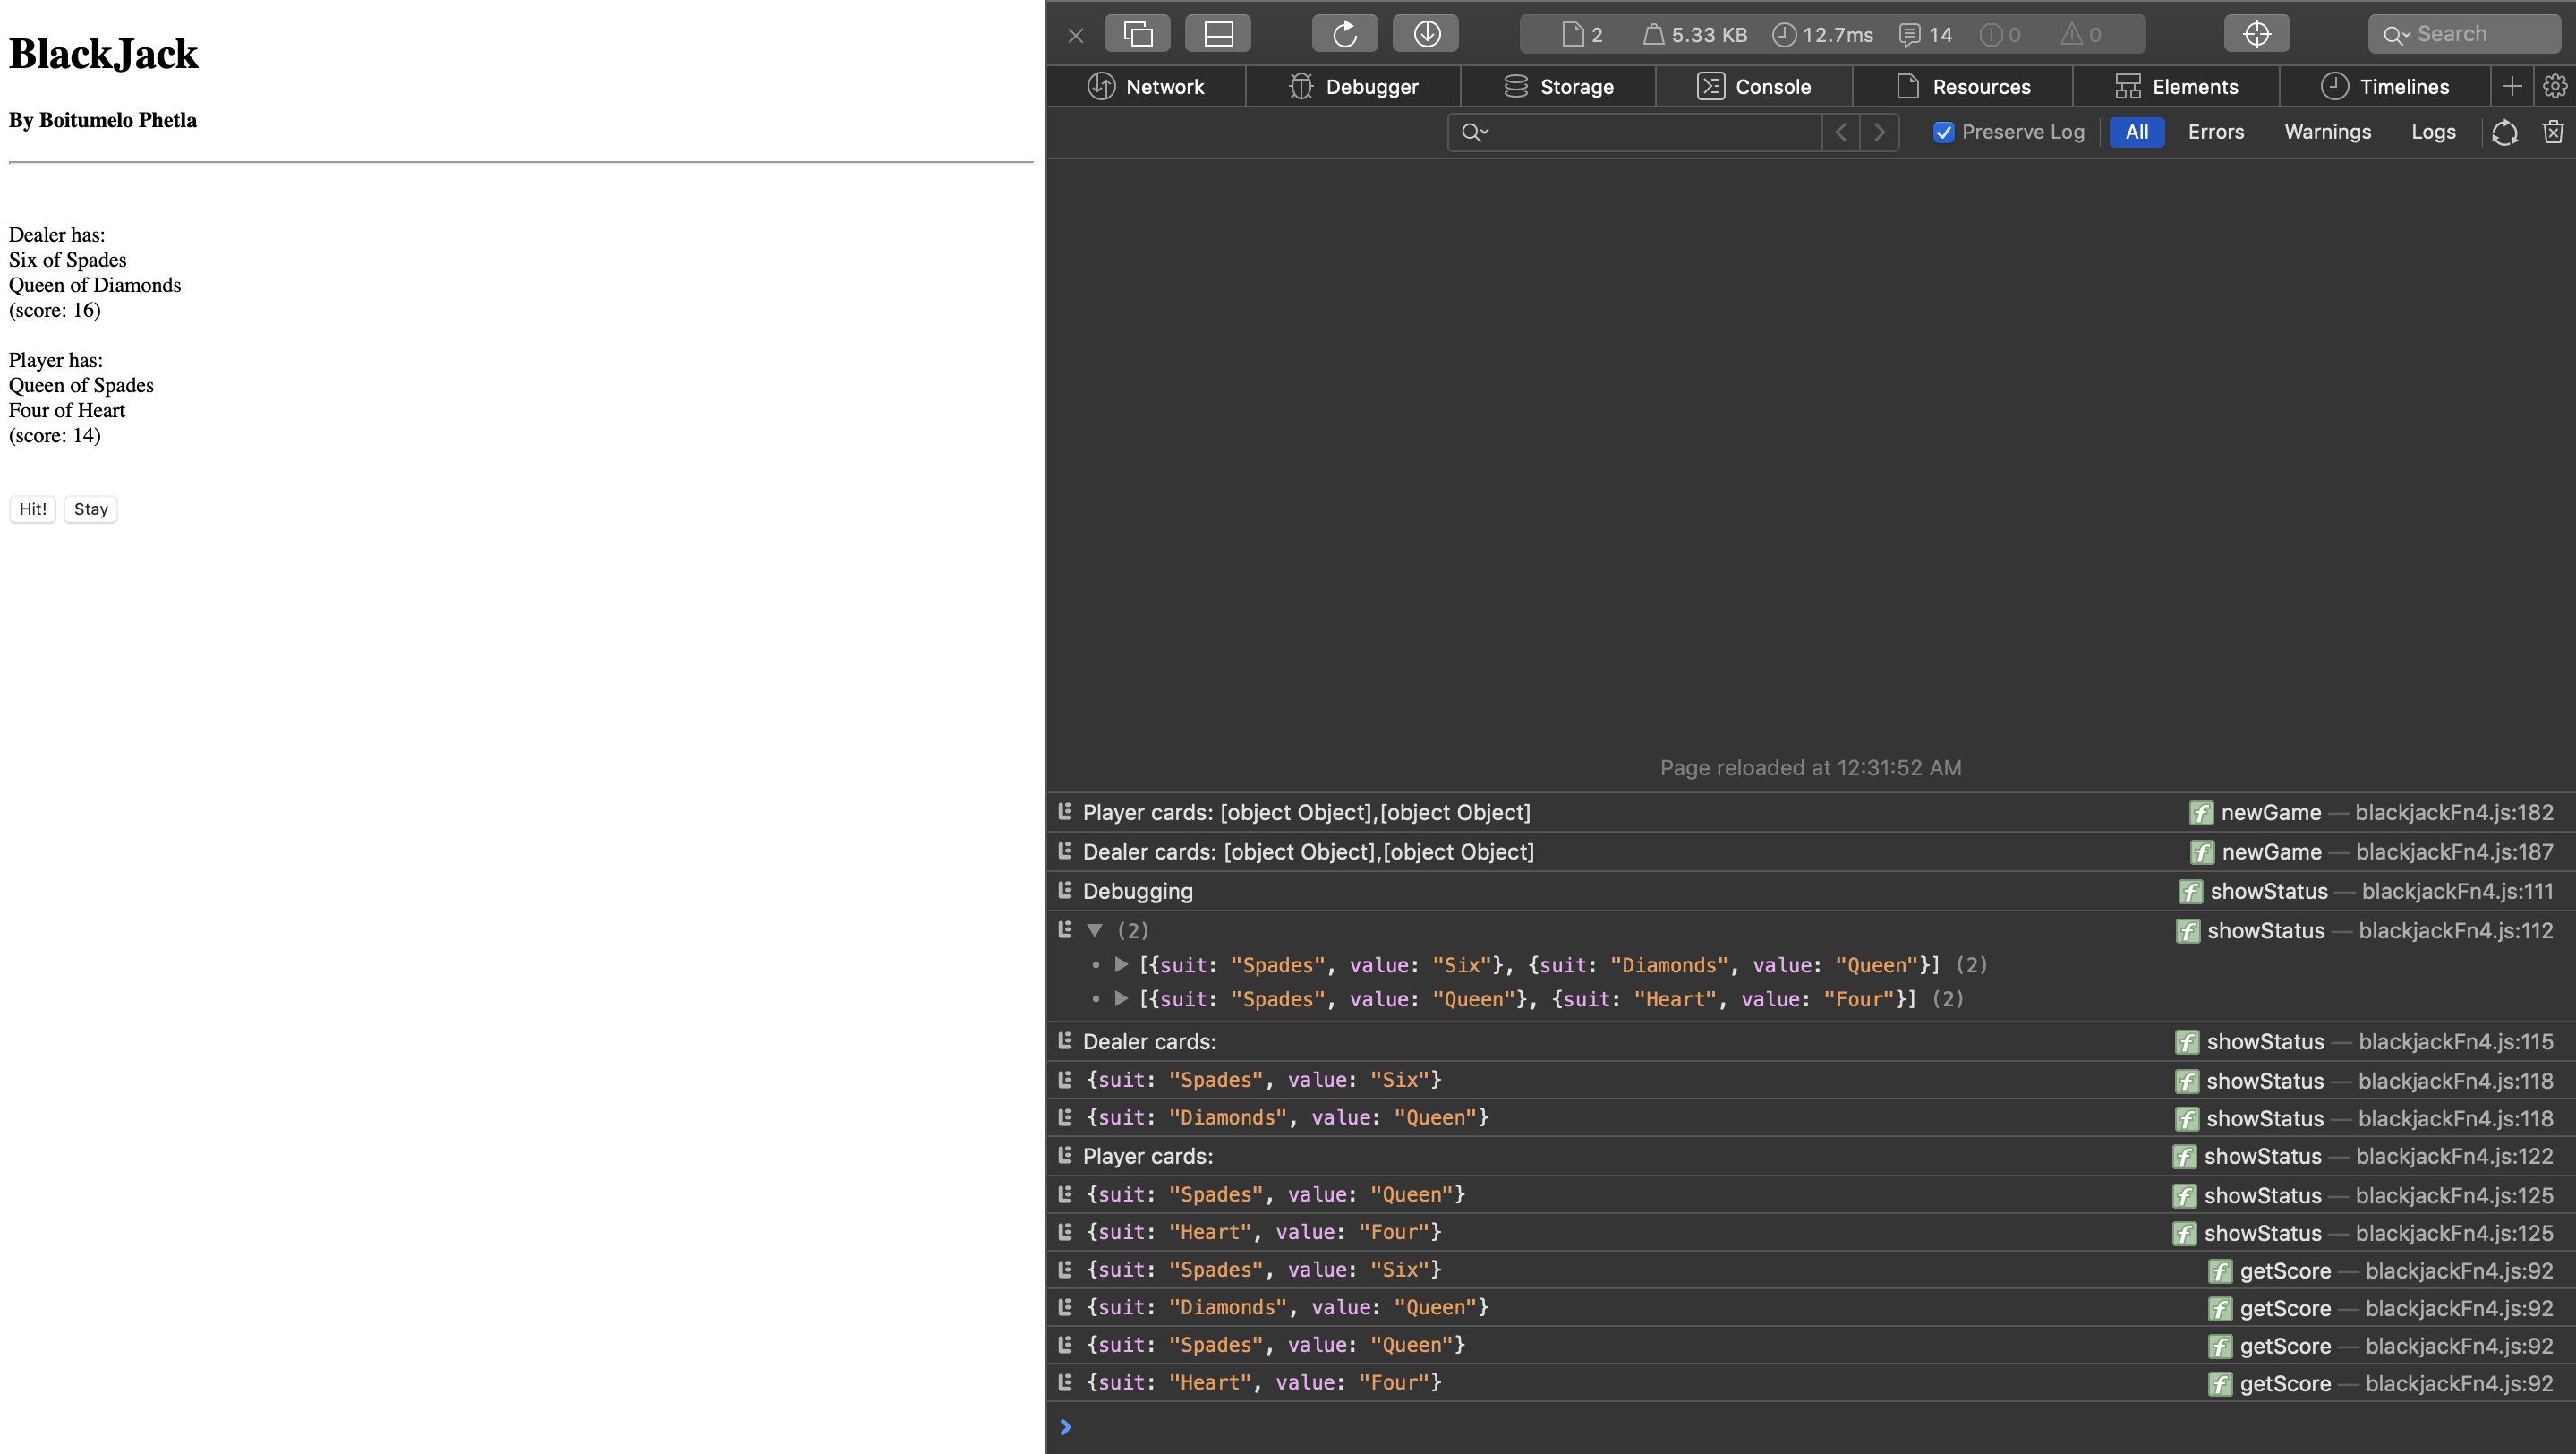
\includegraphics[width=\linewidth]{imgs/dev1.PNG}
	\caption{Game dev status}
	\label{gm}
\end{figure}

\subsection{End of Game}

\begin{lstlisting}
/*
	Blackjack game of cards
*/

//Game variables
let gameStarted = false, gameOver = false, playerWon = false, dealerCards = [], playerCards = [], dealerScore = 0, playerScore = 0, deck = []

//card variables
let suits = ["Heart", "Clubs", "Diamonds", "Spades"];
let values = ["Ace", "King", "Queen", "Jack", "Ten", "Nine", "Eight", "Seven", "Six", "Five", "Four", "Three", "Two"];

//DOM variables
let textArea = document.getElementById('text-area')
let newGameButton = document.getElementById('new-game-button')
let hitButton = document.getElementById('hit-button')
let stayButton = document.getElementById('stay-button')

//create deck function
function createDeck(){
		/*
				Creates a deck of 52 cards
		*/
		let deck = [] //crear deck
		for(let suitIdx = 0; suitIdx < suits.length; suitIdx++){
				for(let valueIdx = 0; valueIdx < values.length; valueIdx++){
						let card = {
										suit : suits[suitIdx],
										value: values[valueIdx]
						}
						deck.push(card);
				}
		}
				return deck
}

function getNextCard(){
		/*Moves to the next card from the card on top*/
		return deck.shift()
}

var getCardString = (card) =>{
		/*
				takes object { suit: "v1", valueL "v2"}
				returns: v2 of v1
		*/
		return card.value + ' of ' + card.suit
}

function hide(object){
		object.style.display = 'none' //remove element
}

function unhide(object){
		object.style.display = 'inline' //revert back
}

function getCardNumericValue(card){
		switch(card.value){
				case 'Ace':
						return 1
				case 'Two':
						return 2
				case 'Three':
						return 3
				case 'Four':
						return 4
				case 'Five':
						return 5
				case 'Six':
						return 6
				case 'Seven':
						return 7
				case 'Eight':
						return 8
				case 'Nine':
						return 9
				default:
						return 10
		}
}

function checkForEndGame(){
		updateScore()

		if(gameOver){
				//let dealer take card
				while(dealerScore < playerScore && playerScore <= 21 && dealerScore <= 21){
								dealerCards.push(getNextCard())
								updateScore()
								alert(dealerScore)
				}
		}

		if(playerScore > 21){
				playerWon = false
				gameOver = true
		}else if(dealerScore > 21){
				playerWon = true
				gameOver = true
		}else if(gameOver){
				if(playerScore > dealerScore){
						playerWon = true
				}else{
						playerWon = false
				}
		}
}

function updateScore(){
		dealerScore = getScore(dealerCards)
		playerScore = getScore(playerCards)
}

function getScore(cardArray){
		let score = 0
		let hasAce = false
		for (var i = 0; i < cardArray.length; i++) {
				let card = cardArray[i]
				console.log(card);
				score += getCardNumericValue(card)
				if(card.value === 'Ace'){
						hasAce = true
				}
		}
		if(hasAce && score + 10 <= 21){
				return score + 10
		}

		return score
}

function showStatus(){
		if(!gameStarted){
				textArea.innerText = "Welcome to BlackJack!"
				return;
		}

		console.log("Debugging")
		console.log(dealerCards, playerCards) //debugging

		let dealerCardString = ''
		console.log("Dealer cards:");
		for (let i = 0; i < dealerCards.length; i++) {
				dealerCardString += getCardString(dealerCards[i]) + '\n'
				console.log(dealerCards[i])
		}

		let playerCardString = ''
		console.log("Player cards:");
		for (let i = 0; i < playerCards.length; i++) {
				playerCardString += getCardString(playerCards[i]) + '\n'
				console.log(playerCards[i])
		}

		updateScore()

		textArea.innerText =
				'Dealer has:\n' +
				dealerCardString +
				'(score: ' + dealerScore + ')\n\n'+

				'Player has:\n' +
				playerCardString +
				'(score: ' + playerScore + ')\n\n'

		if(gameOver){
				if(playerWon){
						textArea.innerText = "You WIN!"
				}else{
						textArea.innerText = "DEALER WINS!"
				}

				unhide(newGameButton)
				hide(hitButton)
				hide(stayButton)
		}


}

//shuffle deck
function shuffleDeck(deckOfCards){
		for(let i = 0; i < deckOfCards.length; i++){
				let swapIdx = Math.trunc(Math.random()* deckOfCards.length)
				let tmp = deckOfCards[swapIdx];
				deckOfCards[swapIdx] = deckOfCards[i]
				deckOfCards[i] = tmp
		}
}


//new game function
function newGame(textObject, newGameButtonObject, hitButtonObject, stayButtonObject){

		gameStarted = true
		gameOver = false    //this is redundant
		playerWon = false

		//create card deck
		deck = createDeck()

		//shuffle deck
		shuffleDeck(deck)

		//player cards
		for(let i = 0; i < 2; i++){
				playerCards.push(getNextCard())
		}
		console.log("Player cards: " + playerCards);
		//dealer cards
		for(let i = 0; i < 2; i++){
				dealerCards.push(getNextCard())
		}
		console.log("Dealer cards: " + dealerCards);

		textObject.innerText = "Started..."
		//hide newGameButton
		hide(newGameButtonObject)
		//unhide stay and hit button
		unhide(hitButtonObject)
		unhide(stayButtonObject)

		//status
		showStatus()
}

//start hide hit and stay button
hide(hitButton)
hide(stayButton)

newGameButton.addEventListener('click', function(){
		newGame(textArea, newGameButton, hitButton, stayButton)
})

hitButton.addEventListener('click', function(){
		playerCards.push(getNextCard())
		checkForEndGame()
		showStatus()
})

stayButton.addEventListener('click', function(){
		gameOver = true
		checkForEndGame()
		showStatus()
})

\end{lstlisting}

\section{Functions}

Simple function.

\begin{lstlisting}
function showMessage(){
		console.log("This is a simple function");
}

showMessage() //This is a simple function
\end{lstlisting}

Passing data into a function.

\begin{lstlisting}
function showMessage(message){
			console.log(message);
}

showMessage("Hello, world!") //Hello, world!

\end{lstlisting}

Return statement in a function.

\begin{lstlisting}
"use strict"

function doubles(number){
		return number*2;
}

var r = doubles(2)
console.log(r); //4
\end{lstlisting}

\section{Objects}

\subsection{Create an Object}

\begin{lstlisting}
"use strict"

//object person
let person = {
		name : "x",
		surname: "y",
		age: 0,
		occupation: "a",
		vehicle: "b"
}

console.log(person); // { name: 'x', surname: 'y', age: 0, occupation: 'a', vehicle: 'b' }
\end{lstlisting}

\subsection{Access an Object}

Accessing hash table object.

\begin{itemize}
	\item Dot notation person.name
	\item by indexing person['name']
\end{itemize}

\begin{lstlisting}
"use strict"

//object person
let person = {
			name : "x",
			surname: "y",
			age: 0,
			occupation: "a",
			vehicle: "b"
}

console.log(person);
/*
	{
			name: 'x',
			surname: 'y',
			age: 0,
			occupation: 'a',
			vehicle: 'b' }
*/

var keys = Object.keys(person)

/*
	[ 'name', 'surname', 'age', 'occupation', 'vehicle' ]
*/

var myInformation = ['John', 'Doe', 29, 'Engineer', 'Porsche 911']

let count = 0 //count values

keys.forEach((key) => {
			person[key] = myInformation[count]
			count++
})

console.log(person);

/*
		{ name: 'John',
		surname: 'Doe',
		age: 29,
		occupation: 'Engineer',
		vehicle: 'Porsche 911' }
*/
\end{lstlisting}

\subsection{Parsing an object into a function}

\begin{lstlisting}
"use strict"

//change card function
var changeCard = (card_) => {
		card_.suit = "Clubs"
}
let card = {
		suit: "Hearts",
		value: "Queen"
}

console.log(card) //{suit: "Hearts", value: "Queen"}
changeCard(card)
console.log(card) //{suit: "Clubs", value: "Queen"}

\end{lstlisting}

\subsection{Arrays of Objects}

\begin{lstlisting}
"use strict"

let cards = [
					{
							suit : "Hearts",
							value: "Queen"
					}
]

console.log(cards) //[ { suit: 'Hearts', value: 'Queen' } ]
console.log(cards[0]) //{ suit: 'Hearts', value: 'Queen' }
console.log(cards[0].suit) //Hearts
\end{lstlisting}

accessing array objects.

\begin{lstlisting}
"use strict"

let cards = [

			{
					suit : "Hearts",
					value: "Queen"
			},

			{
					suit: "Clubs",
					value: "King"
			},

			{
					suit: "Diamonds",
					value: "King"
			}

]

let numberOfCards = cards.length //3
for(let i = 0; i < numberOfCards; i++){
			console.log(cards[i].value + " of " + cards[i].suit)
}

/*
		Queen of Hearts
		King of Clubs
		King of Diamonds
*/

\end{lstlisting}


\subsection{Built-in Objects}

\href{https://developer.mozilla.org/en-US/docs/Web/JavaScript/Reference/Global_Objects}{Standard Built-in Objects}

\begin{description}
	\item[Math] : random numbers
	\item [Date]: date objects
	\item [String]: strings
 	\item [Number]: numbers
\end{description}

\subsection{Math Object}

Simple game.

\begin{lstlisting}
"use strict"

var guess = (number) =>{
		if (number == (Math.random()*10).toFixed(0)){
					console.log("You chose " + number +" JackPot!!!")
		}else{
					console.log("This round: " + number + ", JackPot number: " + (Math.random()*10).toFixed(0))
				}
}

//Guess number between 0 - 10
let guessNumbers = [1,2,3,4,5,6,7,8,9,10]

guessNumbers.forEach((element) => {
			guess(element)
})

//Lost ten times
/*
This round: 1, JackPot number: 7
This round: 2, JackPot number: 7
This round: 3, JackPot number: 9
This round: 4, JackPot number: 6
This round: 5, JackPot number: 7
This round: 6, JackPot number: 0
This round: 7, JackPot number: 7
This round: 8, JackPot number: 5
This round: 9, JackPot number: 1
This round: 10, JackPot number: 3
*/

//Win
/*
	You chose 9 JackPot!!!
*/
\end{lstlisting}

\subsection{Math truncate}

\begin{lstlisting}
"use strict"

//truncate rounds and removes all decimal points
var guess = (number) =>{
			if (number == Math.trunc((Math.random()*10))){
					console.log("You chose " + number +" JackPot!!!")
			}
}

//Guess number between 0 - 10
let guessNumbers = [1,2,3,4,5,6,7,8,9,10]

guessNumbers.forEach((element) => {
		guess(element)
})

/*
	You chose 8 JackPot!!!
*/
\end{lstlisting}

\subsection{Date Object}

\begin{lstlisting}
"use strict"

var date = new Date()
console.log(date); //2019-06-15T19:06:25.648Z

\end{lstlisting}

\subsection{toDateString()}

\begin{lstlisting}
"use strict"

var date = new Date().toDateString()
console.log(date); //Sat Jun 15 2019
\end{lstlisting}

\section{Programming for web pages}

\subsection{DOM}

Document Object Model: Defines how the data of a web page is organized and manipulated.

\begin{description}
	\item[Document] : HTML file
	\item[Model]:  Data (stored in an object)
\end{description}

\subsection{Programming the DOM}

\begin{lstlisting}[language=HTML]
<!DOCTYPE html>
<html>
	<head>
			<title>Listing1</title>
	</head>
			<body>
			<p id="test">DOM</p>

			<script>
							let para = document.getElementById('test')
							console.log(para);
							para.innerText = "Document Object Model"
			</script>
			</body>
 </html>
\end{lstlisting}

\subsection{Accessing DOM objects using an external file}

\begin{description}
	\item[HTML File] : listing2.html
\end{description}
\begin{lstlisting}
<!DOCTYPE html>
<html>
	<head>

			<title>
					Listing2
		  </title>

	</head>
					<body>

							<h1 id="h_1">Listing2</h1>

							<script src="listing2.js"></script>

					</body>
</html>
\end{lstlisting}

\begin{description}
	\item[JS File] : listing2.js
\end{description}

\begin{lstlisting}
"use strict"
//class
function Simple(a,b){
	this.a = a,
	this.b = b
}

//method 1
Simple.prototype.sum = function(){
	return (this.a + this.b)
}

//instantiation
var d = new Simple(12,2)
console.log(d.sum())

//manipulating the DOM
var h = document.getElementById('h_1')
h.innerText = "Version " + (d.sum()).toString()
\end{lstlisting}

\subsection{Handling Buttons}

\begin{description}
	\item[HTML file] : listing3.html
\end{description}

\begin{lstlisting}
<!DOCTYPE html>
<html>
	<head>
			<title>Listing2</title>
	</head>
	<body>
		<h1 id="h_1">Handling Events</h1>
		<p id="formula">Function used here</p>
		<button type="button" name="ok-button" id="ok_button">OK</button>
		<script src="listing3.js"></script>
	</body>
</html>
\end{lstlisting}

\begin{description}
	\item[JS file] : listing3.js
\end{description}

\begin{lstlisting}
"use strict"

let ok_Button = document.getElementById('ok_button')

function M(a,b){
		this.a,
		this.b
}

M.prototype.sum = function(){
		//sum() method from class M(a,b)
		return this.a + this.b
}

ok_Button.addEventListener('click', function(){
		//code here...
		let ff = new M(2,3)
		var f = document.getElementById('formula')
		f.innerText = ff.sum //get function
})

\end{lstlisting}

\subsection{Manipulating DOM object styles}

\begin{description}
	\item[HTML file]: listing4.js
\end{description}

\begin{lstlisting}
<!DOCTYPE html>
<html>
	<head>
			<title>Listing2</title>
	</head>
	<body>
		<h1 id="h_1">Handling Events</h1>
		<p id="text">Manipulate this text</p>
			<button type="button" name="ok-button" id="clear">
					clear
			</button>
			<button type="button" name="revert-button" id="revert">
				Revert
			</button>
		<script src="listing4.js"></script>
	</body>
</html>
\end{lstlisting}

\begin{description}
	\item[JS file]: listing4.js
\end{description}

\begin{lstlisting}
"use strict"

var clear_button = document.getElementById('clear')
var revert_button = document.getElementById('revert')
var textToManipulate = document.getElementById("text")

function clear(object){
		object.style.display = 'none' //remove element
}

function revert(object){
		object.style.display = 'block' //revert element
}

clear_button.addEventListener('click', function(){
		clear(textToManipulate)
})

revert_button.addEventListener('click', function(){
		revert(textToManipulate)
})
\end{lstlisting}
\printbibliography[title={Bibliography}] % Print the bibliography, section title in curly brackets

%----------------------------------------------------------------------------------------

\end{document}
